\chapter{Concept}
\label{ch:concept}

\section{Présentation}
\label{sec:concept_introduction}

Un VESAD est une technique d'extension d'un écran physique par RA : un visiocasque de RA affiche une fenêtre virtuelle placée automatiquement autour d'écran physique que l'on souhaite étendre, sur le même plan que lui. En synchronisant ces deux affichages, l'utilisateur peut alors voir et interagir avec comme s'il s'aggissait d'un seul écran étendu. Cette technique peut ainsi être appliquée pour tout type d'écran, incluant ceux des ordinateurs, les télévisions ou les affichages muraux. Nous travaillons cependant seulement avec l'extension de l'écran d'un téléphone intelligent, notre premier sous-problème étant de concevoir l'IHM d'un VESAD sur un téléphone : nous la situons d'abord par rapport à la littérature, puis nous décrivons quelques applications et techniques d'interactions potentielles.

Notre IHM s'incrit dans la continuité de plusieurs travaux. Elle d'abord rend concret le concept de bureau de travail en RA Desktop Gluey \citep{Serrano2015a} dont nous implémentons donc le cas où les fenêtres virtuelles sont alignées avec un écran physique mobile. Cela correspond au mode \texten{device-aligned} dans MultiFi \citep{Grubert2015}, dont nous reprenons l'idée d'écrans étendus par RA. Elle est enfin un cas particulier du Personal Cockpit \citep{Ens2014} où nous situons la fenêtre virtuelle non pas par rapport au corps mais autour du téléphone.

Nous situons donc notre IHM en utilisant le cadre de conception Ethereal Planes \citep{Ens2014a}. Cela est pertinent car nous concevons une IHM sous forme d'une fenêtre 2D dans un environnement de RA. La \reffigureETS{VesadInEtherealPlanes} montre qu'un télephone étendu par un VESAD suit les caractéristiques de la catégorie \texten{palette} pour le cadre de référence et la composition spatiale. Cependant, nous souhaitons comparer une technique d'interaction utilisant l'écran tactile (catégorie \texten{palette}) à une main virtuelle (catégorie \texten{floating}) dans notre évaluation expérimentale.

\figureLayoutETS{VesadInEtherealPlanes}{%
  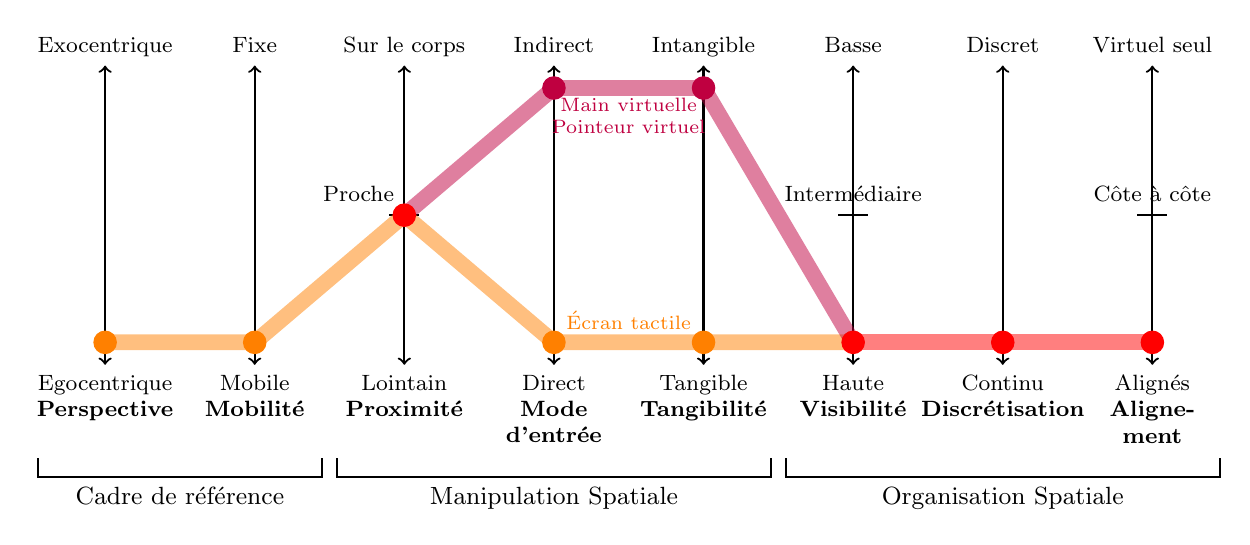
\begin{tikzpicture}[font=\footnotesize, scale=0.95]
    \tikzstyle{dimension}=[thick, <->]
    \tikzstyle{etiquetteb}=[below, align=center, text depth=.25ex]
    \tikzstyle{etiquettea}=[above, align=center, text depth=.25ex]

    \draw[thick] (-0.9,-1.25) -- (-0.9,-1.5) -- (1,-1.5) node[etiquetteb] {\small Cadre de référence} -- (2.9,-1.5) -- (2.9,-1.25);
    \draw[dimension] (0,0) node[etiquetteb] {Egocentrique\\\textbf{Perspective}} -- (0,4) node[etiquettea] {Exocentrique};
    \draw[dimension] (2,0) node[etiquetteb] {Mobile\\\textbf{Mobilité}} -- (2,4) node[etiquettea] {Fixe};

    \draw[thick] (3.1,-1.25) -- (3.1,-1.5) -- (6,-1.5) node[etiquetteb] {\small Manipulation Spatiale} -- (8.9,-1.5) -- (8.9,-1.25);
    \draw[dimension] (4,0) node[etiquetteb] {Lointain\\\textbf{Proximité}} -- (4,4) node[etiquettea] {Sur le corps};
    \draw[thick] (3.8,2) -- (4,2) node[etiquettea, above left] {Proche} -- (4.2,2);
    \draw[dimension] (6,0) node[etiquetteb] {Direct\\\textbf{Mode}\\\textbf{d'entrée}} -- (6,4) node[etiquettea] {Indirect};
    \draw[dimension] (8,0) node[etiquetteb] {Tangible\\\textbf{Tangibilité}} -- (8,4) node[etiquettea] {Intangible};

    \draw[thick] (9.1,-1.25) -- (9.1,-1.5) -- (12,-1.5) node[etiquetteb] {\small Organisation Spatiale} -- (14.9,-1.5) -- (14.9,-1.25);
    \draw[dimension] (10,0) node[etiquetteb] {Haute\\\textbf{Visibilité}} -- (10,4) node[etiquettea] {Basse};
    \draw[thick] (9.8,2) -- (10,2) node[etiquettea] {Intermédiaire} -- (10.2,2);
    \draw[dimension] (12,0) node[etiquetteb] {Continu\\\textbf{Discrétisation}} -- (12,4) node[etiquettea] {Discret};
    \draw[dimension] (14,0) node[etiquetteb] {Alignés\\\textbf{Aligne-}\\\textbf{ment}} -- (14,4) node[etiquettea] {Virtuel seul};
    \draw[thick] (13.8,2) -- (14,2) node[etiquettea] {Côte à côte} -- (14.2,2);

    \tikzstyle{ligne}=[line width=0.2cm, opacity=0.5]
    \draw[ligne, orange] (0,0.3) -- (2,0.3) -- (4,2) -- (6,0.3) -- (8,0.3) -- (10,0.3);
    \draw[ligne, purple] (4,2) -- (6,3.7) -- (8,3.7) -- (10,0.3);
    \draw[ligne, red] (10,0.3) -- (12,0.3) -- (14,0.3);

    \draw[orange] (7,0.3) node[etiquettea, font=\scriptsize] {Écran tactile};
    \draw[purple] (7,3.7) node[etiquetteb, font=\scriptsize] {Main virtuelle\\Pointeur virtuel};

    \draw[orange, fill=orange] (0,0.3) circle[radius=0.15];
    \draw[orange, fill=orange] (2,0.3) circle[radius=0.15];
    \draw[red, fill=red] (4,2) circle[radius=0.15];
    \draw[orange, fill=orange] (6,0.3) circle[radius=0.15];
    \draw[purple, fill=purple] (6,3.7) circle[radius=0.15];
    \draw[orange, fill=orange] (8,0.3) circle[radius=0.15];
    \draw[purple, fill=purple] (8,3.7) circle[radius=0.15];
    \draw[red, fill=red] (10,0.3) circle[radius=0.15];
    \draw[red, fill=red] (12,0.3) circle[radius=0.15];
    \draw[red, fill=red] (14,0.3) circle[radius=0.15];
  \end{tikzpicture}%
}{
  Évaluation de notre IHM de téléphone étendu par un VESAD avec notre version d'Ethereal Planes : il suit la catégorie \texten{palette} (en orange), sauf pour le mode d'entrée et la tangibilité où nous proposons plusieurs techniques d'interactions utilisées dans les catégories \texten{palette} et \texten{floating} (en violet). Quand ces deux catégories se recoupent, on utilise le rouge.
}

En outre, nous avons ajouté une nouvelle dimension à ce cadre. Le mode d'alignement de MultiFi \citep{Grubert2015} décrit le placement de la fenêtre virtuelle, à la fois par rapport à l'utilisateur et par rapport au téléphone ou à la montre intelligente ainsi que les interactions possibles. Cette description est un peu floue et mélange en réalité les dimensions de perspective et de mode d'entrée du cadre avec une nouvelle dimension que nous appelons \emph{alignement}. Cette dernière permet de répondre à la question de l'alignement virtuel-réel dans la définition d'\cite{Azuma1997}. En effet, en suivant l'échelle de \cite{Milgram1994}, on imagine qu'un espace de travail en RA permet de :
\begin{itemize}
  \item travailler seulement avec des fenêtres virtuelles sans lien avec des objets ou écrans physiques comme avec le Personal Cockpit ou le HoloLens (virtuel seul);
  \item utiliser ensemble des fenêtres virtuelles et des objets ou écrans physiques, sans qu'il n'y ait de relations spatiales entre eux, comme dans Gluey ou Desktop-Gluey (côte à côte);
  \item étendre, joindre et augmenter des objets ou écrans physiques avec des fenêtres virtuels, comme avec MultiFi ou notre VESAD (alignés).
\end{itemize}
\bigskip

Ainsi, toutes ces IHMs d'espace de travail en RA que nous venons de citer dans ce chapitre sont compatibles et complémentaires. Nous les imaginons donc comme différents modes d'un seul système d'exploitation utilisant un visiocasque de RA à large champ de vision (haute visibilité) et les appareils intelligents disponibles. Nous les présentons sur le \autoref{tab:ar_os} : un tel système d'exploitation proposerait l'alignement avec les écrans physiques que souhaite l'utilisateur, dans tous les cadres de références et toutes les proximités possibles. La discrétisation contrôle à quel point l'information est fragmentée sur les écrans virtuels et physiques utilisés, ou s'ils forment un affichage continu. Plusieurs techniques d'interactions devraient être disponibles mais nous faisons l'hypothèse que certaines sont plus adaptées que d'autres en fonction du mode utilisé et du contexte d'utilisation.

Dans ce mémoire, nous explorons, implémentons, et évaluons donc seulement une technique d'alignement (écrans étendus ou VESAD) dans la continuité de MultiFi. Le téléphone étant tenu en main, il s'agit d'un cadre egocentrique mobile.

\begin{tableETS}{tab:ar_os}{Correspondance des différentes IHMs de la \autoref{sec:litterature_ar_worspaces} dans les dimension perspective, mobilité et alignement (avec des écrans physiques) de notre version d'Ethereal Planes.}
  \begin{tabular}{ccc|*{3}{c|}}
    \cline{4-6} & & & \multicolumn{3}{c|}{\textbf{Alignement}} \\
    \cline{4-6} & & & \textbf{Virtuel seul} & \textbf{Côte à côte} & \textbf{Alignés} \\
    \hline \multicolumn{1}{|c|}{\multirow{4}{*}{\rotatebox{90}{\shortstack{\textbf{Cadre de}\\\textbf{référence}}}}} & \multicolumn{1}{c|}{\multirow{2}{*}{\textbf{Exocentrique}}} & \textbf{Fixe} & \multirow{2}{*}{HoloLens} & \multirow{4}{*}{\shortstack{Gluey /\\ Desktop Gluey}} & \multirow{4}{*}{\shortstack{VESAD /\\ MultiFi}} \\
    \cline{3-3} \multicolumn{1}{|c|}{} & \multicolumn{1}{c|}{} & \textbf{Mobile} & & & \\
    \cline{2-4} \multicolumn{1}{|c|}{} & \multicolumn{1}{c|}{\multirow{2}{*}{\textbf{Egocentrique}}} & \textbf{Fixe} & \multirow{2}{*}{Personal Cockpit} & & \\
    \cline{3-3} \multicolumn{1}{|c|}{} & \multicolumn{1}{c|}{} & \textbf{Mobile} & & & \\
    \hline
  \end{tabular}
\end{tableETS}


\section{Applications potentielles}
\label{sec:concept_applications}

Nous distinguons deux modes de vues, correspondants à la dimension discrétisation d'Ethereal Planes, pour afficher du contenu dans un téléphone à écran étendu :
\begin{itemize}
  \item Vue multi-fenêtres : de multiples applications utilisées conjointement sont placées sur l'écran physique et le reste de l'écran étendu \reffigureETSp{HandheldVESADApp}.
  \item Vue étendue : une seule application utilise tout l'écran étendu \reffigureETSp{HandheldVESADExtended}.
\end{itemize}
\bigskip

\figureLayoutETS{HandheldVESADApp}{%
  \subfigureETS{HandheldVESADApps.jpg}{Plusieurs applications ainsi que des notifications détaillée sont affichées dans la fenêtre virtuelle en parallèle à celle sur l'écran physique.}%
  \figurehspace%
  \subfigureETS{HandheldVESADApps2.jpg}{Wrist : une rotation de la main permet de rapidement changer l'application sur l'écran physique.}%
}{
  Photomontages d'un téléphone à écran étendu en vue multi-fenêtres, où de multiples applications se partagent l'écran étendu.
}

En vue multi-fenêtres, l'utilisateur peut donc interagir avec de multiples applications en même temps comme sur un ordinateur, qu'il organise librement, ou de manière plus structurée selon une grille, sur l'écran étendu. L'écran d'accueil du téléphone pourrait ainsi montrer l'ensemble des applications installées, ou en cours d'exécution \reffigureETSp{HandheldVESADApps.jpg} permettant à un utilisateur de facilement changer l'application affichée sur l'écran physique. Un autre cas d'utilisation est des prises de notes d'un cours ou d'une conférence : autour d'une application de notes sur l'écran physique, l'utilisateur pourrait placer la vidéo de l'intervention ainsi que les diapositives sur la droite de l'écran, et plusieurs onglets de pages web ou de références pour compléments d'informations sur la gauche. Il peut alors aller et venir d'un regard de ces notes, à la vidéo ou aux références, comme on peut le faire sur un ordinateur.

La fenêtre virtuelle peut également être utilisée par le système d'exploitation du téléphone par exemple pour afficher des informations plus détaillées que sur la barre de notifications en haut de l'écran, ou la barre des tâches d'un ordinateur : par exemple le nom et le sujet des messages et courriels non-lus, une liste des prochains événements du calendrier ou un graphique de l'état de la batterie depuis le dernier chargement \reffigureETSp{HandheldVESADApps.jpg}. La zone en bas de l'écran peut elle être mise à profit pour visualiser la liste des données (texte, images) copiées par l'utilisateur et lui permettre de facilement sélectionner ce qu'il veut coller ; cette opération est difficile avec les IHMs des téléphones actuels. Enfin, en exploitant la 3D -- en débordant donc du cadre d'une fenêtre virtuelle -- les notifications pourraient s'accumuler en piles l'arrière du téléphone : une rotation similaire à la \reffigureETS{HandheldVESADApps2.jpg} permettrait alors de les visualiser complètement.

\figureLayoutETS{HandheldVESADExtended}{%
  \subfigureETS{HandheldVESADMap.jpg}{Une carte de navigation.}%
  \figurehspace%
  \subfigureETS{HandheldVESADDogs.jpg}{Une galerie d'images.}%
  \figurehspace%
  \subfigureETS{HandheldVESADTooltip.jpg}{Info-bulles dans la fenêtre virtuelle.}%
}{
  Photomontages d'applications en vue étendue, exploitant tout l'écran étendu du VESAD.
}

En vue étendue, une application occupe tout l'espace d'affichage. L'utilisateur peut souhaiter par exemple voir une vue plein écran d'une application, une page web ou une carte de navigation en exploitant la totalité de l'écran étendu \reffigureETSp{HandheldVESADMap.jpg}. Cela permet de ainsi visualiser un large document, ou une version pour ordinateur dans le cas d'une page web. Une application peut également utiliser l'écran étendu pour structurer son information : par exemple, une application de messagerie afficherait la conversation courante sur l'écran physique avec dans la fenêtre virtuelles les fichiers échangés dans cette conversation ainsi que la liste des contacts. Enfin, un navigateur web pourrait afficher autour de l'onglet courant sur l'écran physique la liste des onglets ouverts dans la fenêtre virtuelle : les gestes avec un doigt agissent sur l'écran physique tandis que ceux à deux doigts agissent sur l'écran étendu, par exemple pour faire défiler de gauche à droite les onglets ouverts, vers le bas pour fermer le courant, vers le haut pour le mettre en favoris ; des interactions directes avec une main virtuelles seraient aussi possibles.

Une application peut également se servir de la fenêtre virtuelle pour afficher des informations en relation avec l'écran physique, comme des infobulles d'aide \reffigureETSp{HandheldVESADTooltip}, des commentaires sur un document PDF ou encore des interfaces de contrôle d'une vidéo ou d'une musique jouée. À l'inverse, \cite{Grubert2015} proposent d'utiliser un clavier sur tout l'écran physique en affichant le texte tapé dans une fenêtre virtuelle.

Enfin, on peut mettre en \oe uvre des techniques de visualisation comme Overview+Detail ou Focus+Context sur l'écran étendu. La vue détaillée peut être affichée sur l'écran physique ou sur la fenêtre virtuelle. Par exemple, la \reffigureETS{HandheldVESADDogs.jpg} montre une image détaillé dans la fenêtre virtuelle (\texten{detail}) sélectionnée depuis une galerie d'images affichée sur l'écran physique (\texten{overview}). Ces deux vues peuvent donc être inversées, par exemple pour profiter de la haute définition de l'écran physique.


\section{Techniques d'interactions}
\label{sec:concept_interaction_techniques}

Une de nos questions de recherche \autorefp{sec:research_problem} est quelle technique d'interaction est la plus adaptée pour un téléphone étendu par un VESAD. On peut en effet penser à différentes techniques qui ont été explorées dans la littérature pour interagir avec telle IHM :

\begin{itemize}
  \item Pointer directement le contenu avec une main virtuelle, utilisé par le Personal Cockpit \cite{Ens2014} et exploré par \cite{Piumsomboon2013}.
  \item Utiliser l'écran tactile du téléphone, comme dans la condition \condition{Smartwatch referenced} de MultiFi \citep{Grubert2015} ou dans une application ARCore ou ARKit.
  \item Utiliser un pointeur virtuel et des gestes de sélection \cite{Wilson2006}, comme sur un Microsoft HoloLens.
  \item Via des commandes vocales, évaluées par \cite{Piumsomboon2014}.
\end{itemize}
\bigskip

Cette question est ouverte car elle n'a été étudié que par \cite{Grubert2015}. Or les concepts de \cite{Serrano2015} puis \cite{Serrano2015a}, dont nous prenons la suite avec le VESAD, proposent de laisser à l'utilisateur d'utiliser comme il le souhaite les dispositif d'entrées et sorties disponibles. Comme nous évaluons le cas particulier d'un téléphone à écran étendu, nous souhaitons donc savoir si une technique d'interaction semble la plus adaptée.

Nous avons dans le \autoref{ch:litterature} que le pointage direct utilisant une main virtuelle était difficile \citep{Chan2010}. En particulier, \cite{Ens2014} ont montré qu'une main virtuelle était plus stable et moins sujette aux erreurs avec des fenêtres virtuelles placées dans un cadre exocentrique plutôt qu'egocentrique. Cependant, un téléphone à écran étendu étant tenu en main, on peut considérer que la fenêtre est alors placée dans l'environnement de manière stable, même si mobile, plutôt que par rapport au corps de l'utilisateur.

\figureETS{HandheldVESADSlideToHang.jpg}{
  Un geste Slide to Hang permet à un utilisateur de détacher une application de l'écran étendu pour la fixer en l'air, contre une surface ou relativement à son corps. Dans ce photomontage, un utilisateur détache dans un premier temps une page web en l'air, puis un lecteur vidéo.
}

En outre, nous présentons deux nouvelles techniques d'interactions pour notre IHM :
\begin{enumerate}
  \item Wrist : un mouvement de la main tenant le téléphone permet de changer rapidement l'affichage sur l'écran physique dans une vue multi-fenêtres. La \reffigureETS{HandheldVESADApps2.jpg} montre par exemple l'utilisateur tournant son téléphone à \ang{90} environ vers la droite pour changer l'application affichée sur l'écran physique. Un pointeur virtuel suivant le regard ou la tête de l'utilisateur permettrait de choisir l'application sur l'ecran virtuel à utiliser, par exemple parmi une liste d'icônes d'applications.
  \item Slide to Hang : un geste de glissement permet de détacher une fenêtre de l'écran étendu et la fixer en l'air. La \reffigureETS{HandheldVESADSlideToHang.jpg} montre l'utilisateur faisant un geste de glissement (\texten{slide} en anglais) sur le téléphone pour fixer en l'air la fenêtre qui y est affichée. La fenêtre peut être alors placée à un endroit fixe sur un mur ou en l'air, comme avec le HoloLens, ou relativement à son propre corps, comme dans le Personal Cockpit \cite{Ens2014}. Ce geste de glissement peut se faire avec deux doigts simultanément sur le téléphone pour distinguer d'actions faites sur l'application, ou avec un pincement des doigts sur l'écran virtuel \cite{Piumsomboon2014}. Un geste de pincement similaire ramenant la fenêtre fixée vers l'écran étendu permettrait de la ramener relative au téléphone. Cette technique est particulièrement importante car elle permet de déplacer du contenu de l'écran étendu vers des fenêtres dans l'environnement, et donc de rendre compatible le VESAD avec les autres modes du \autoref{tab:ar_os}.
\end{enumerate}